\section{Project Planning}
Prior to starting development, the requirements were estimated and the
development split into several iterations, each driven by a requirement.
Figure~\ref{gantt} shows the initial planning of the development.

\begin{figure}[htb]
  \centering
  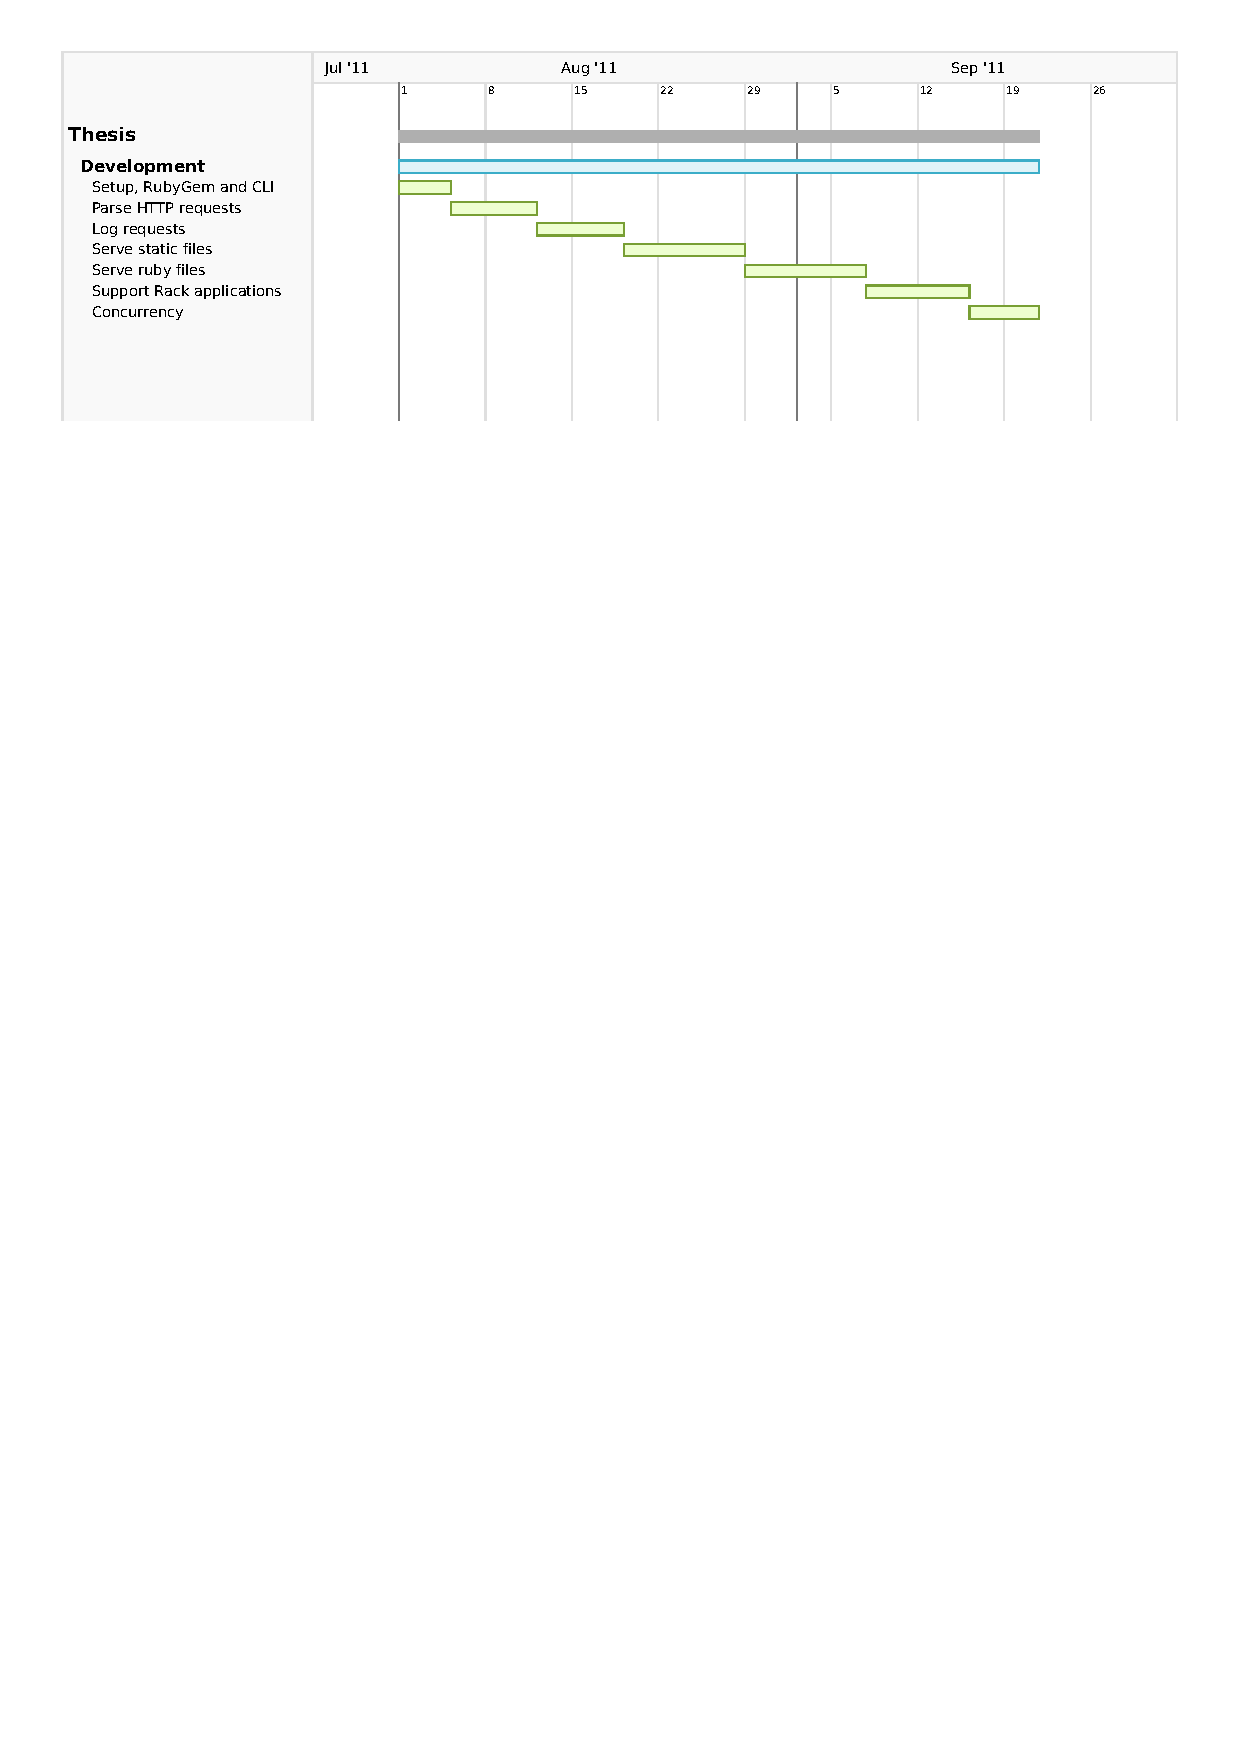
\includegraphics[width=1.0\textwidth]{img/gantt.pdf}
  \caption{Development Gantt Planning}
  \label{gantt}
\end{figure}

The development was planned to take place between August 1 and September 20.
The first three days were to be spent setting up the project, RubyGems
packaging and writing the command-line interface (CLI). Each requirement is
then implemented in turn, with varying time set aside, depending on the
complexity of the task.

As Behaviour-Driven Development was being used, no design was needed upfront,
and development could start head on. Design and architectural decisions were
to be made once the need arose, and tests were to be written prior to any
functionality.
